\documentclass{article}
\usepackage{graphicx}
\usepackage{amsfonts}
\begin{document}
\author{Prabath Peiris  \\ AIND Term 1 \\ Udacity}
\date{}
\title{Experiment with Air Cargo Problem}
\maketitle

\section*{Implement a Planning Search}


All the Air Cargo problems uses the following action schema

\begin{verbatim}
Action(Load(c, p, a),
	PRECOND: At(c, a) ∧ At(p, a) ∧ Cargo(c) ∧ Plane(p) ∧ Airport(a)
	EFFECT: ¬ At(c, a) ∧ In(c, p))

Action(Unload(c, p, a),
	PRECOND: In(c, p) ∧ At(p, a) ∧ Cargo(c) ∧ Plane(p) ∧ Airport(a)
	EFFECT: At(c, a) ∧ ¬ In(c, p))

Action(Fly(p, from, to),
	PRECOND: At(p, from) ∧ Plane(p) ∧ Airport(from) ∧ Airport(to)
	EFFECT: ¬ At(p, from) ∧ At(p, to))
\end{verbatim}

\subsection*{Part 1 - Planning problems}
\subsubsection*{Uniformed Search Strategies}
Uniformed searched strategies does not have any additional information about states beyond that provided in the problem definition. This is the reason this search strategy also known as blind search. All these uninformed searches do is generate successors and distinguish a goal state from a non-goal state. In this section, I compare the performance of 3 different strategies in terms of speed (execution time, measured in seconds), memory usage (measured in search node expansions) and optimality (Yes, if a solution of optimal length is found; No, otherwise).

\begin{table}[h]
\begin{center}
\begin{tabular}{|l|l|l|l|}
\hline
{\tt air\_cargo\_p1} & Breadth First & Depth First Graph& Uniform Cost Search \\ \hline\hline
Node Expansions& 43 & 12 & 55\\ 
Goal Tests & 56 & 13 & 57\\ 
Time Elapsed& 0.053 & 0.015 & 0.064\\ 
Optimality & Yes & Yes & Yes\\ \hline
\end{tabular}
\end{center}
\caption{Metrixs for non-huristic planning solution searches for {\tt air\_cargo\_p1}}
\label{tbl:p1p1}
\end{table}

\begin{table}[h]
\begin{center}
\begin{tabular}{|l|l|l|l|}
\hline
{\tt air\_cargo\_p2} & Breadth First & Depth First Graph& Uniform Cost Search \\ \hline\hline
Node Expansions& 3401  & 350 &4761 \\ 
Goal Tests & 4672 & 351 & 4763\\ 
Time Elapsed& 20.8 & 2.2 & 18.36\\ 
Optimality & Yes & No & Yes\\ \hline
\end{tabular}
\end{center}
\caption{Metrixs for non-huristic planning solution searches for {\tt air\_cargo\_p2}}
\label{tbl:p1p2}
\end{table}

\begin{table}[h]
\begin{center}
\begin{tabular}{|l|l|l|l|}
\hline
{\tt air\_cargo\_p2} & Breadth First & Depth First Graph& Uniform Cost Search \\ \hline\hline
Node Expansions& 14491  &  3491& 17615 \\ 
Goal Tests & 17947& 3492  & 17617 \\ 
Time Elapsed& 147.28 &71.8  & 76.0 \\ 
Optimality & Yes & No & Yes\\ \hline
\end{tabular}
\end{center}
\caption{Metrixs for non-huristic planning solution searches for {\tt air\_cargo\_p3}}
\label{tbl:p1p3}
\end{table}
\subsubsection*{Analysis}

Table \ref{tbl:p1p1} to \ref{tbl:p1p3} show the metric for uniformed planning searches for {\tt air\_cargo\_p1, air\_cargo\_p2, air\_cargo\_p3} problems. By looking at the all the metrics, we can see not all the search methods does not give us the optimal result. Depth first graph search for problem 2 and third does not reach optimal search. Given the execution time, the Uniform cost search provide the optimal search results during this experiment.
\begin{figure}[h]
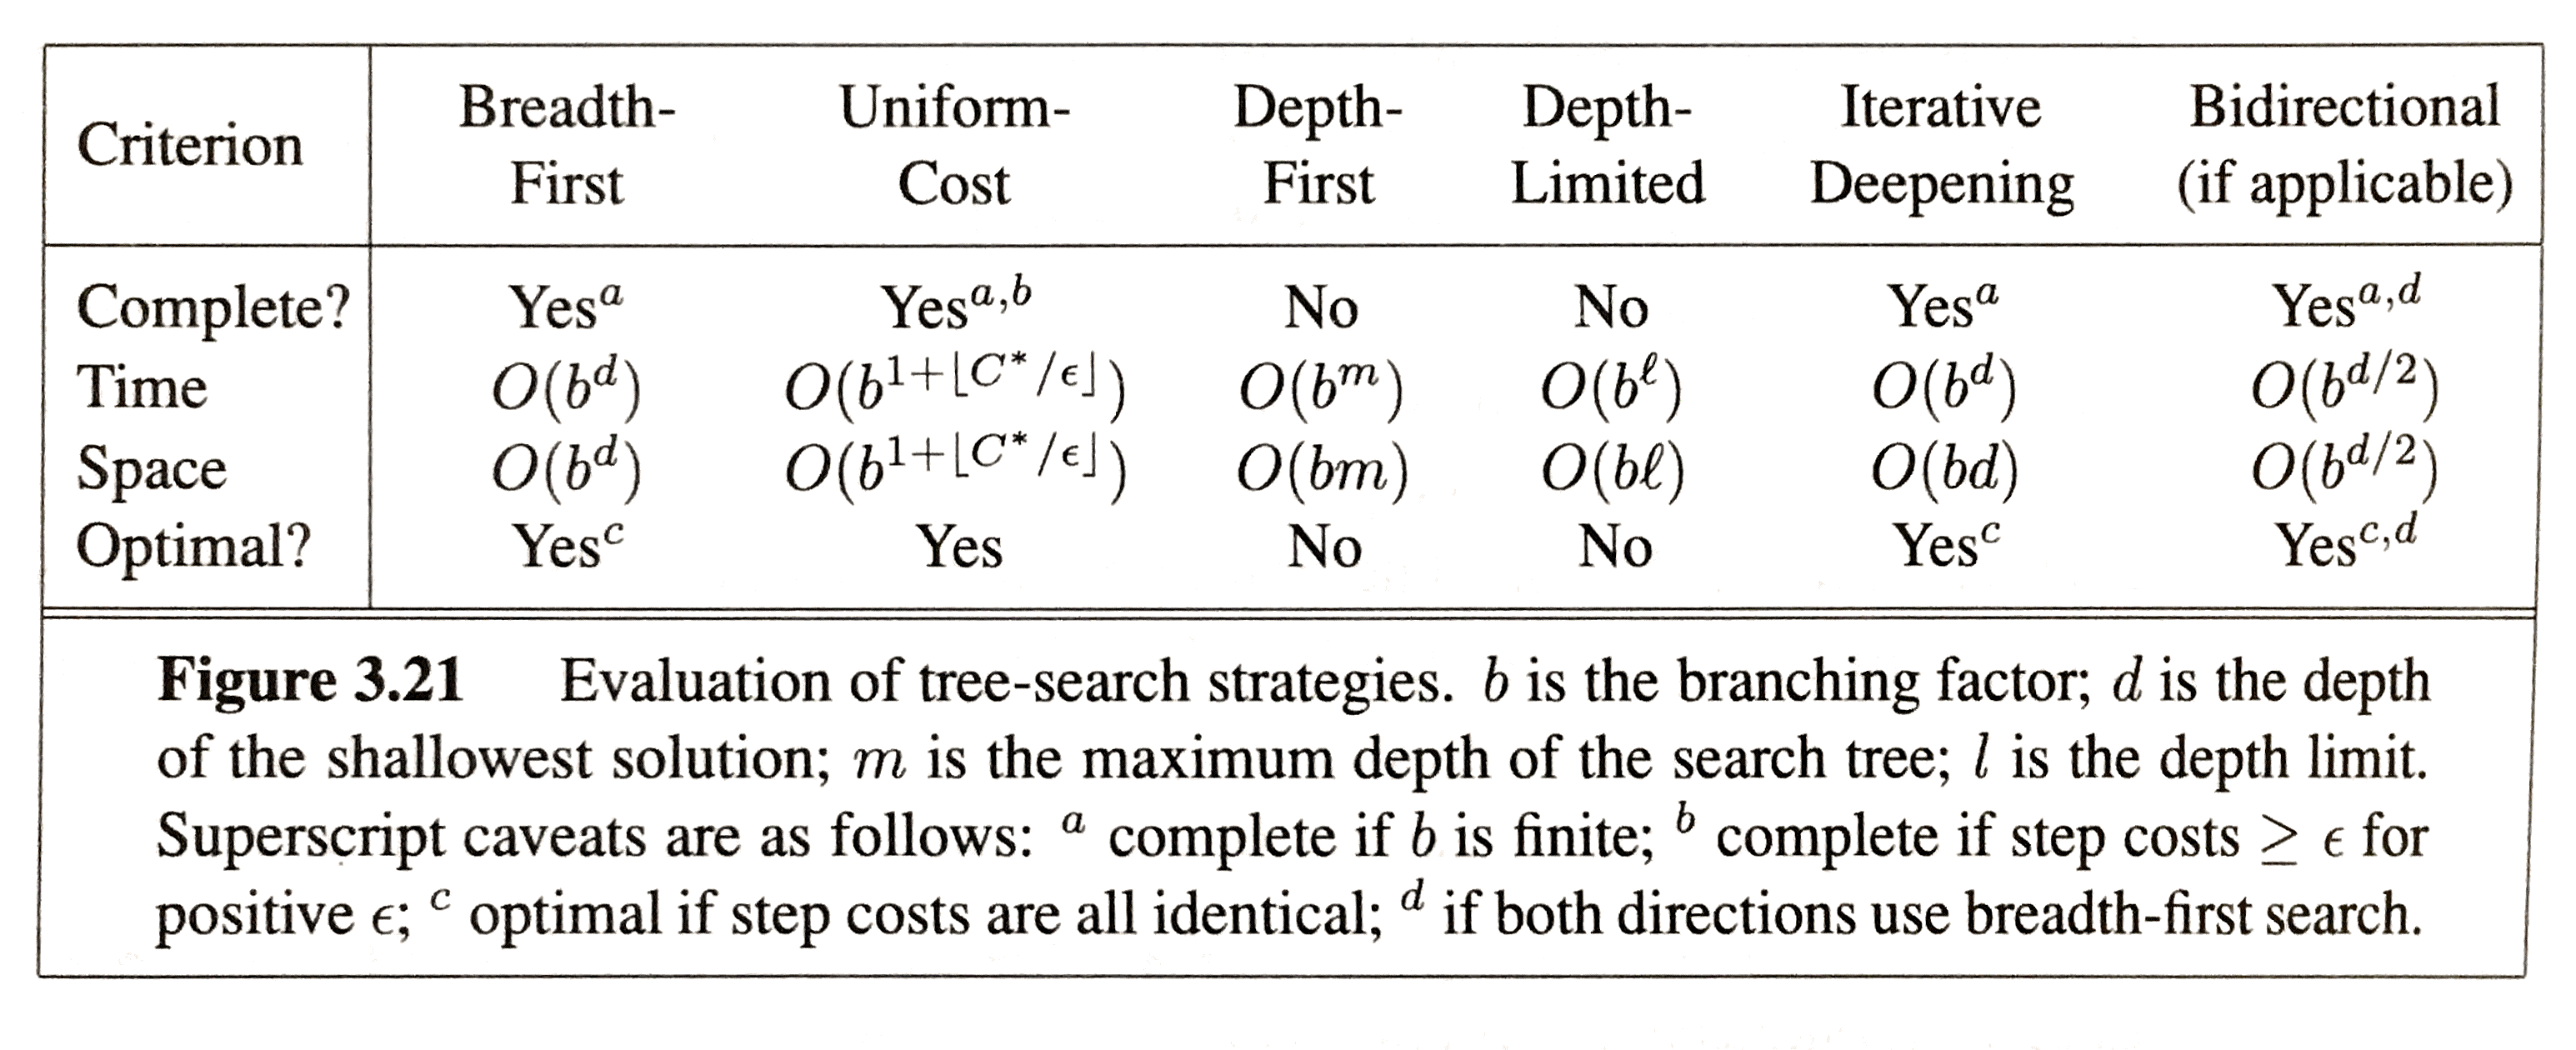
\includegraphics[width=\textwidth]{search}
\end{figure}

Figure 3.21 show the summary of each search methods including its time complexity. Given this information, I can defend my choose of uniform cost search as the optimal by looking at the execution time; however, give the memory usage some can argue the breadth first search may give us the optimal results. This is a valid argument; however, in my defense, I can argue the even memory usage is less with breadth first search, memory itself may not be a game-changing factor when it compares to the execution time. 



\subsection*{Part 2 - Domain-independent heuristics:}

\subsubsection*{Analysis}
Table \ref{tbl:p2p1}  to  \ref{tbl:p2p3} shows the problems {\tt air\_cargo\_p1, air\_cargo\_p2 and air\_cargo\_p3} with 3 different heuristics functions. All the functions reach the optimal solution including the {\tt A* search with level sum heuristic} even it took over 10min to run (took 22 minutes. data left black in table 3 ).  By looking at all the running times of each function, it is evident the {\tt  A* search with ignore predictions heuristic} perform the best.


\begin{table}[h]
\begin{center}
\begin{tabular}{|l|l|l|l|}
\hline
{\tt air\_cargo\_p1} & A* (h1 heuristic) & A* (ignore predictions heuristic) & A* (level sum heuristic)\\ \hline\hline
Node Expansions& 55  &  41 & 11 \\ 
Goal Tests & 57 & 43  & 13 \\ 
Time Elapsed& 0.06 & 0.06  & 1.8 \\ 
Optimality & Yes & Yes & Yes \\ \hline
\end{tabular}
\end{center}
\caption{metrics of A* searches for {\tt air\_cargo\_p1}}
\label{tbl:p2p1}
\end{table}

\begin{table}[h]
\begin{center}
\begin{tabular}{|l|l|l|l|}
\hline
{\tt air\_cargo\_p1} & A* (h1 heuristic) & A* (ignore predictions heuristic) & A* (level sum heuristic)\\ \hline\hline
Node Expansions& 4761  & 1450  & 86 \\ 
Goal Tests & 4763 & 1452  & 88 \\ 
Time Elapsed& 18.3 & 6.9  & 277 \\ 
Optimality & Yes & Yes & Yes \\ \hline
\end{tabular}
\end{center}
\caption{metrics of A* searches for {\tt air\_cargo\_p2}}
\label{tbl:p2p2}
\end{table}

\begin{table}[h]
\begin{center}
\begin{tabular}{|l|l|l|l|}
\hline
{\tt air\_cargo\_p1} & A* (h1 heuristic) & A* (ignore predictions heuristic) & A* (level sum heuristic)\\ \hline\hline
Node Expansions& 17615  &  4728 & -- \\ 
Goal Tests &17617  &  4730 & -- \\ 
Time Elapsed& 77 & 25  & -- \\ 
Optimality & Yes & Yes & -- \\ \hline
\end{tabular}
\end{center}
\caption{metrics of A* searches for {\tt air\_cargo\_p3}}
\label{tbl:p2p3}
\end{table}


\subsection*{Conclusion}
Results are shown in this report demonstrate the advantages using informed search methods with some custom heuristics functions over uninformed search methods when looking for an optimal plan. The benefits are justifiable by looking at both speed (time it took to execute) and the memory usage. It is possible to variate these two measurements to find the best possible search method for given problem which is not feasible with uninformed searches. 


\end{document}
